\section{Dataset}
\label{sec:dataset}
% \todo[inline]{Layout (also text arrangements!), Image of the statistics bigger or different?}

The dataset contains images of 22 different throwing objects, as shown in table \ref{tab:objects}.
It is fully labeled and consists of more than \num{15000} usable images with at least 480 images of each object.
All images were collected over the course of two days.
Figure \ref{subfig:stuffed_bunny} shows an example image of the \textit{Stuffed Bunny} and figure \ref{subfig:hand_featherball} shows an image of the \textit{Hand Featherball}.

Figure \ref{fig:statistics} shows the statistics.
It is evident that there are generally more images of larger objects.
This is, on the one hand, due to the specific implementation of the throw detection mechanism (see section \ref{subsec:throw_detection_mechanism}).
On the other hand, the field of view is not uniformly illuminated, as described in section \ref{subsec:Lighting}.
For those reasons, a larger object area is required at the borders to achieve a sufficiently large change in the image.
However, this also leads to the fact that larger objects are more often only partially in the picture.

An important thing is that, on the first day, the white balance was performed continuously (every three images).
This caused the background color of large colored objects to be distorted.
It remains to be seen whether this will become a problem during training.
However, if this should become a problem, the respective images can easily be removed, as the labels contain a Unix timestamp (see section \ref{subsec:database}).

\begin{table}[hb]
  \caption{List of the different throwing objects}
  \label{tab:objects}
  \centering
  \begin{tabular}{lll}
    \toprule
    \textbf{Objects} &  &  \\
    \midrule
	Nerf Dart & Spiky Ball & Stuffed Bunny \\
	American Football & Tesafilm & Goalkeeper Glove \\
	Table Tennis Ball & Sponge & Hemp Cord \\
	Shuttlecock & Lego Duplo Brick (Red) & Paper Ball \\
	Sporf & Lego Duplo Brick (Green) & Beer Cap \\
	Arrow & Lego Duplo Figure & Water Bottle \\
	Hand Featherball & Foam Dice &  \\
	Floorball & Infant Shoe &  \\
    \bottomrule
  \end{tabular}
\end{table}

\begin{figure}[hb]
  \centering
  \begin{subfigure}[b]{0.45\textwidth}
    \centering
    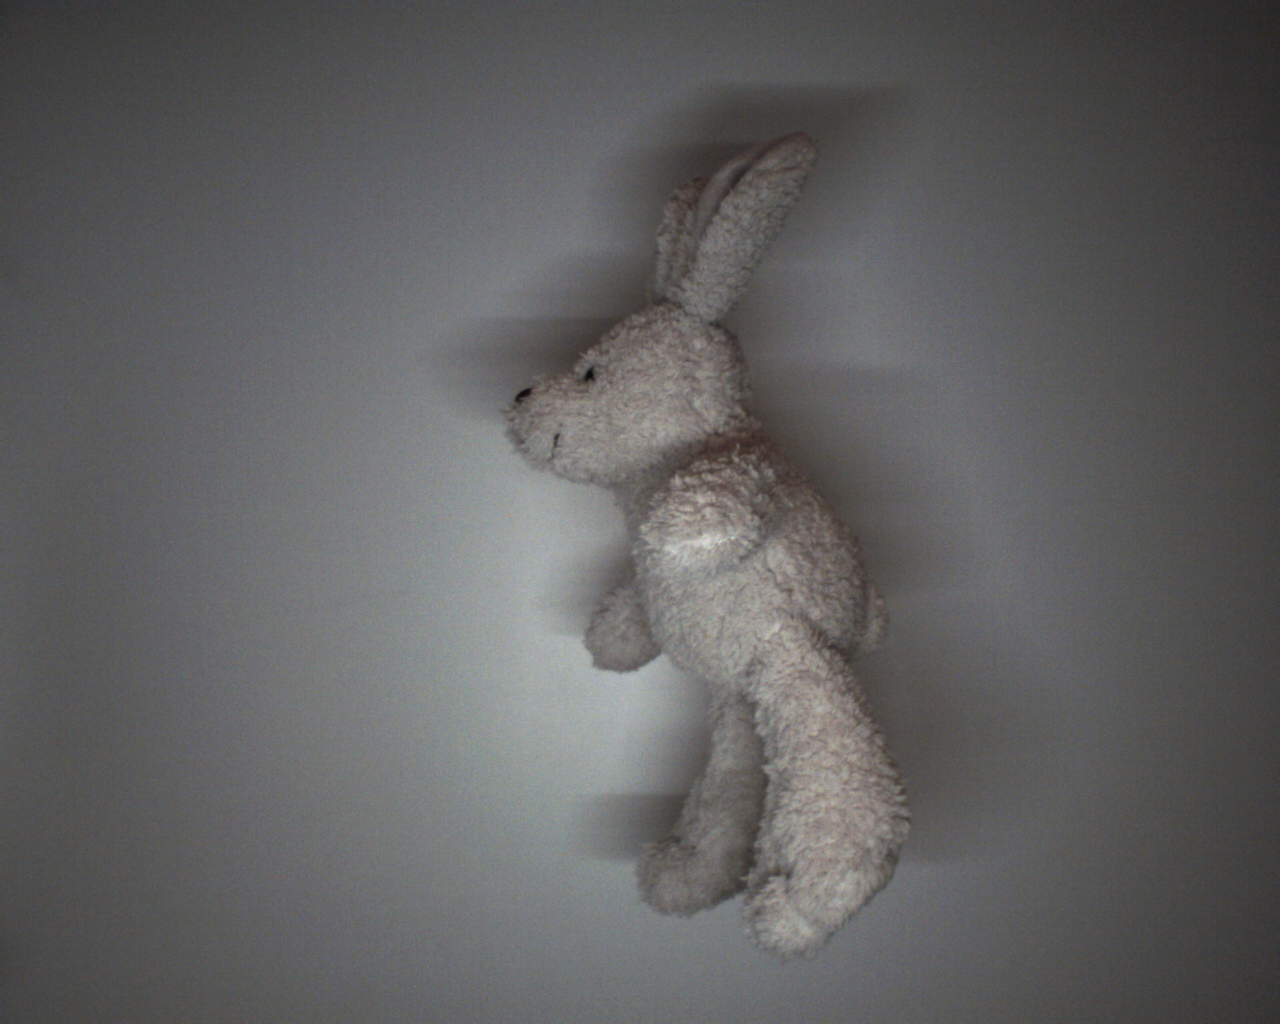
\includegraphics[width=0.9\textwidth]{1574952009_278_10_stuffed-bunny}
    \caption{Stuffed Bunny}
    \label{subfig:stuffed_bunny}
  \end{subfigure}
  \begin{subfigure}[b]{0.45\textwidth}
    \centering
    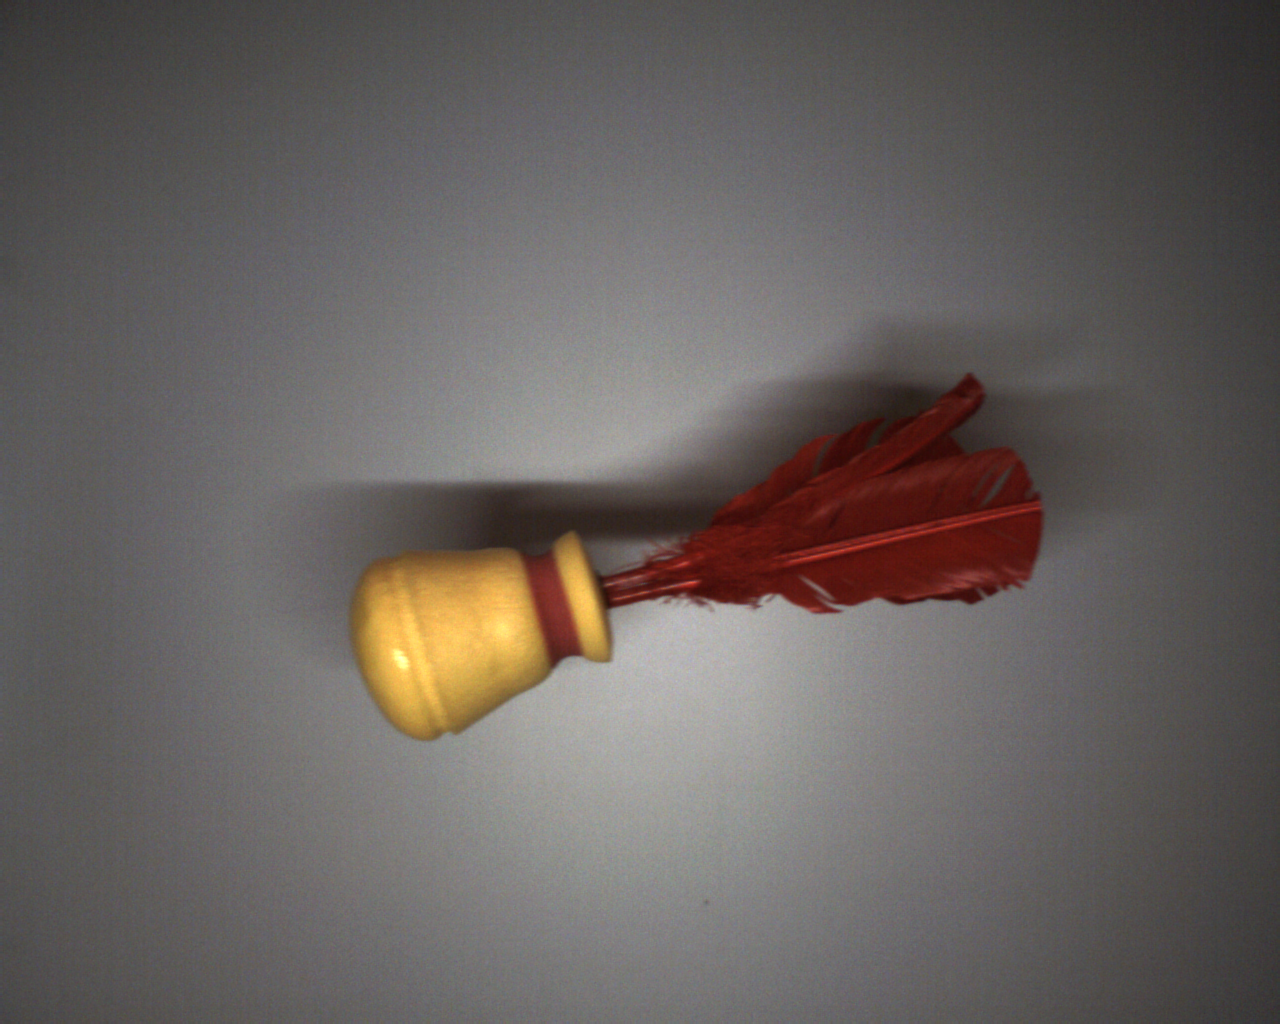
\includegraphics[width=0.9\textwidth]{1574943825_125_8_hand-featherball}
    \caption{Hand Featherball}
    \label{subfig:hand_featherball}
  \end{subfigure}
  \caption{Two pictures from the dataset}
  \label{fig:dataset}
\end{figure}

\begin{figure}[h]
  \centering
  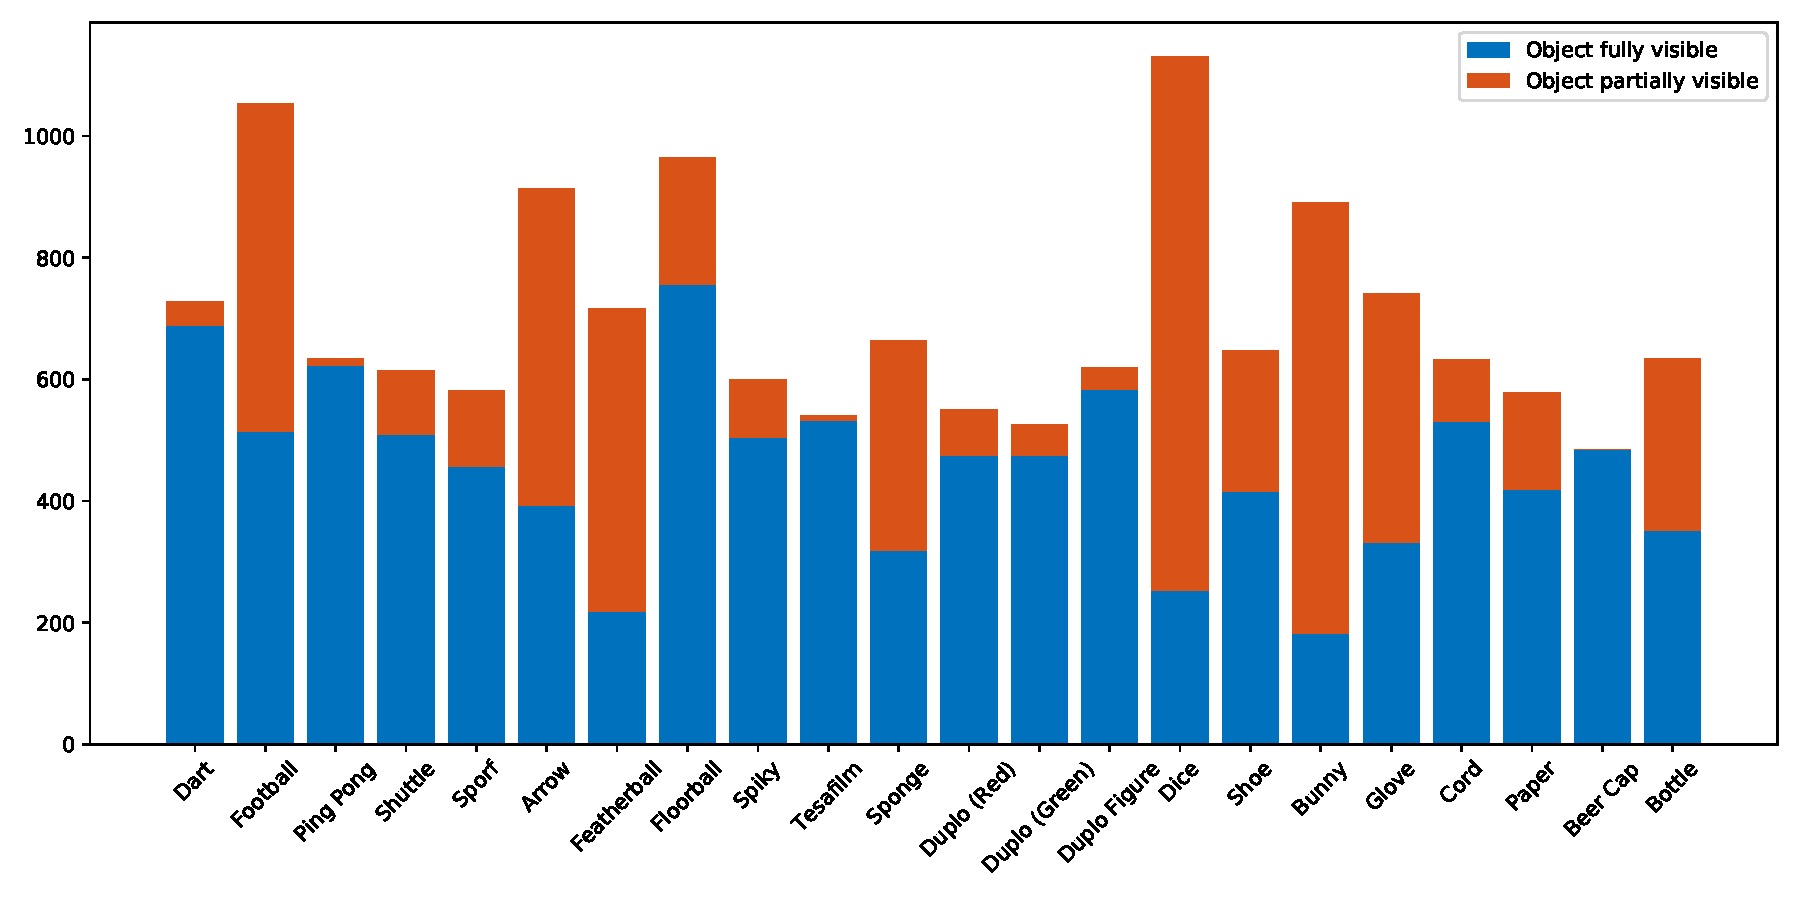
\includegraphics[width=\textwidth]{statistics}
  \caption{Statistics showing the amount of captured frames for each object individually}
  \label{fig:statistics}
\end{figure}

\begin{figure}[h]
  \centering
  \begin{subfigure}[b]{0.45\textwidth}
    \centering
    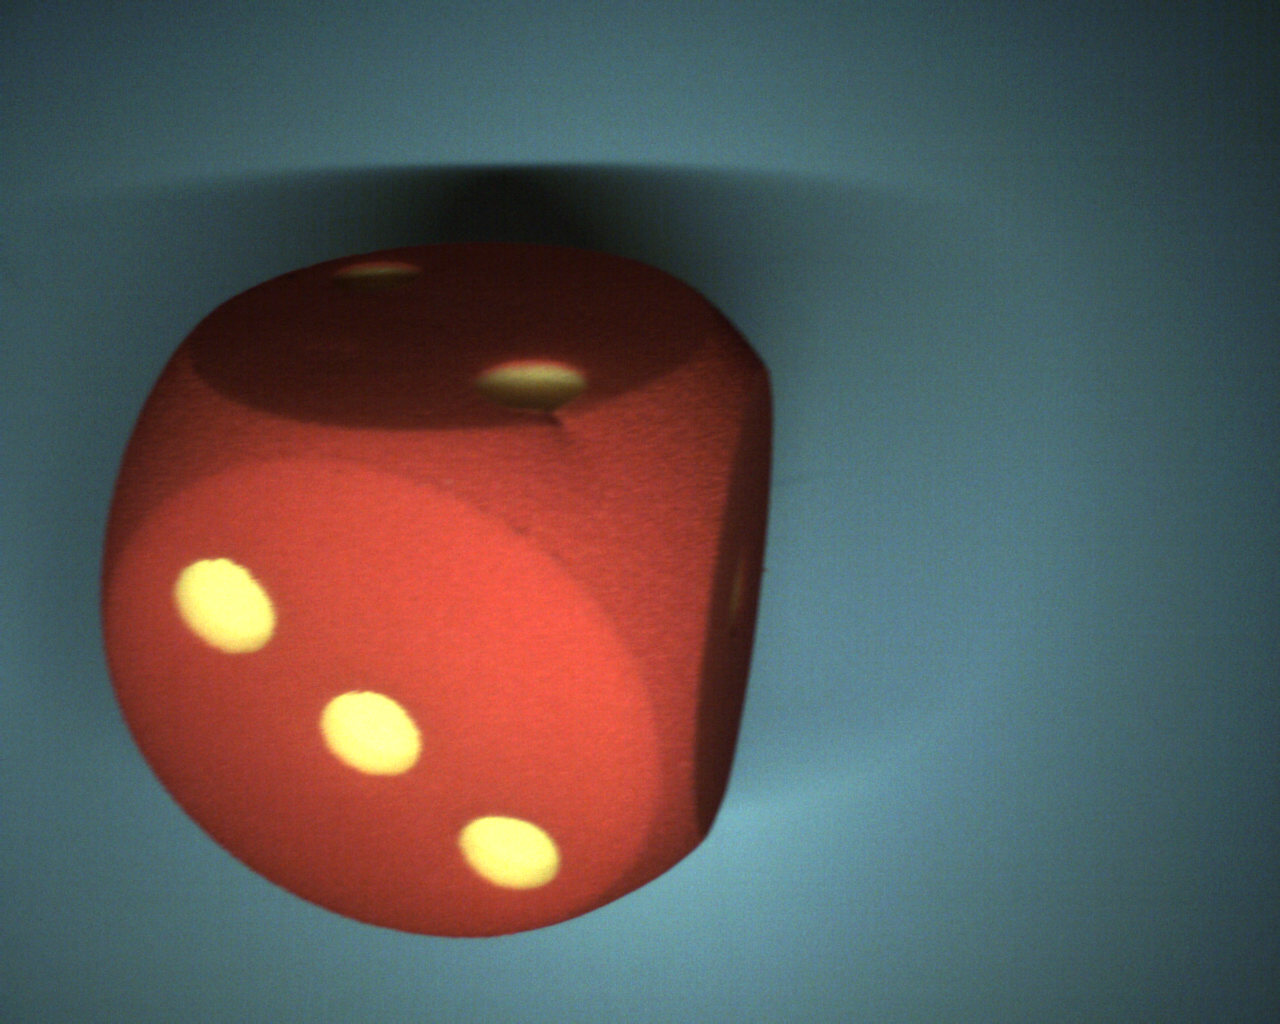
\includegraphics[width=0.9\textwidth]{1574950250_238_9_foam-dice}
    \caption{Continuous white balance}
    \label{subfig:foam_dice_first_day}
  \end{subfigure}
  \begin{subfigure}[b]{0.45\textwidth}
    \centering
    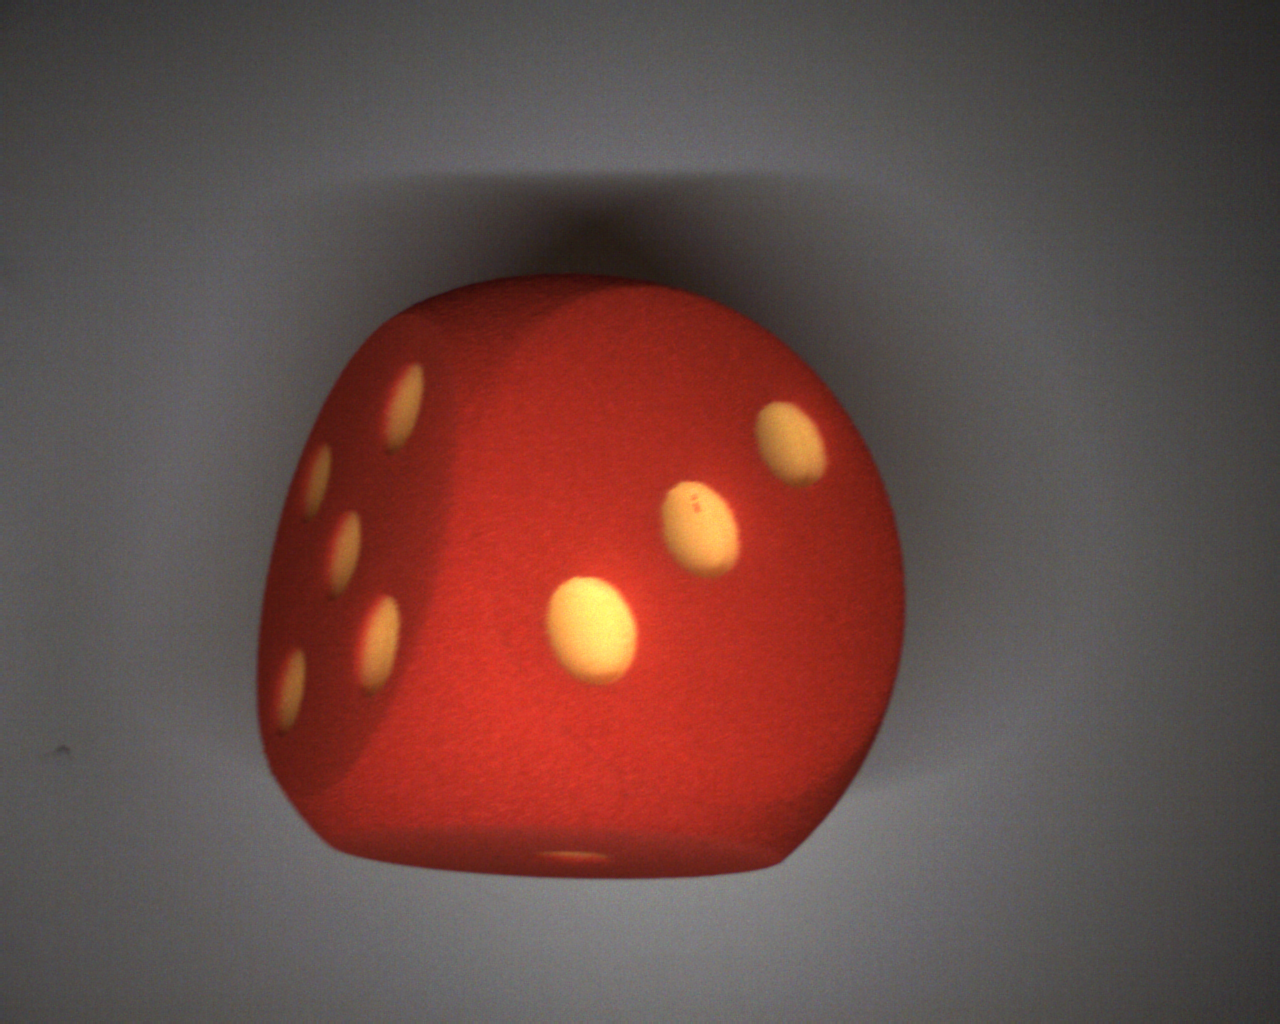
\includegraphics[width=0.9\textwidth]{1575032343_726_11_foam-dice}
    \caption{One-off white balance}
    \label{subfig:foam_dice_second_day}
  \end{subfigure}
  \caption{White balance difference between the first (\subref{subfig:foam_dice_first_day}) and the second (\subref{subfig:foam_dice_second_day}) day}
  \label{fig:dataset_white_balance}
\end{figure}
